\subsection{Description du cas de test}
Le bain initial correspond à un bain oxyde avec une masse initiale de 10 T, une température initiale de 2900 K et une composition de 0.77 UO$_2$ - 0.12 Zr - 0.11 ZrO$_2$ (ratio molaire $R_{U/Zr}$ = 1.3 et degré d'oxydation du zirconium $C_{Zr}$ = 30 \%). La puissance résiduelle constante $\dot{\mathcal{Q}} = 200$ MW est portée par l'espèce uranium U. Une condition adiabatique est imposée sur la couche supérieure du bain. Les propriétés physiques des couches du bain sont calculés en fonction de la composition et de la température de la couche par un code externe (ref ?). Enfin, les caractéristiques utiles des différentes couches du bain sont détaillées dans le tableau~\ref{tab:caracteristiques_couches_bain}, en particulier les températures de \textit{liquidus} $T^{fus}$ ainsi que les corrélations de flux de chaleur utilisées pour le calcul des puissances latérales $\phi S$ (voir~\cite{Bonnet1999} ou~\cite{Tourniaire2009a} pour plus de détails sur les corrélations).
\begin{table}
	\centering
	\begin{tabular}{ccc} 
	\hline
	Couche & $T^{fus}$ (K) & Corrélation latérale\\
	\hline
	Acier liquide (FE.) & 1800 & ChurchillAndChu\\
	Métal léger (LM.) & 1800 & ChurchillAndChu\\
	Oxyde (OX.) & 3000 & BaliDownWard\\
	Métal lourd (HM.) & 1800 & BaliDownWard\\
	\hline
	\end{tabular}	
	\caption{Configuration initiale du bain de corium pour le test.} 
	\label{tab:caracteristiques_couches_bain}
\end{table}

Différentes coulées d'acier liquide à différents instants du calcul permettent de reproduire des stratifications du bain d'intêret pour les calculs accidents graves. En particulier, ces coulées ont été calculées en fonction du seuil d'inversion de stratification du bain (correspondant à quantité d'acier dans la bain permettant le passage d'un état d'équilibre thermochimique composé d'une couche de métaux lourds en dessous d'une couche d'oxydes vers un équilibre composé d'une couche d'oxydes en dessous d'une couche de métaux légers). Les caractéristiques de ces coulées (temps de début et de fin, masse, température et composition) sont détaillés dans le tableau~\ref{tab:coulees_acier}. 
\begin{table}
	\centering
	\begin{tabular}{ccccc} 
	\hline
	$t_{\text{début}}$ (s) &  $t_{\text{arrêt}}$ (s) & Débit (kg/s) & T (K) & Composition\\
	\hline
	800 & 1000 & 8 & 1805 & 0.687 Fe - 0.208 Cr - 0.106 Ni\\
	16000 & 16200 & 8 & 1805 & 0.687 Fe - 0.208 Cr - 0.106 Ni\\
	\hline
	\end{tabular}	
	\caption{Les différentes coulées d'acier liquide imposées pour le test.} 
	\label{tab:coulees_acier}
\end{table}
Un temps suffisament long entre chacune de ces coulées est imposé pour permettre au bain d'atteindre un état quasi-stationnaire de thermique et de thermochimie. Les différentes configurations quasi-stationnaires du bain obtenues (OX. puis HM./OX. puis OX./LM.) sont décrites dans la figure~\ref{fig:stratifications_bains}.
\begin{figure}
\centering
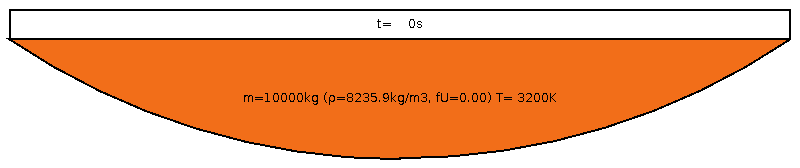
\includegraphics[width=0.85\textwidth, keepaspectratio=true]{Figures/coriumPool_t=00000.png}\\
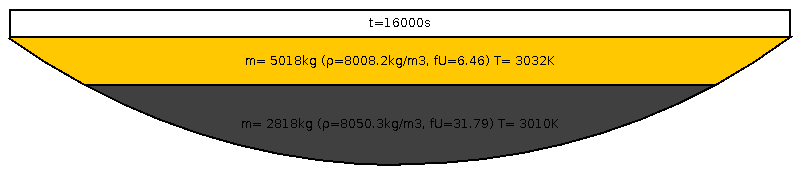
\includegraphics[width=0.85\textwidth, keepaspectratio=true]{Figures/coriumPool_t=16000.png}\\
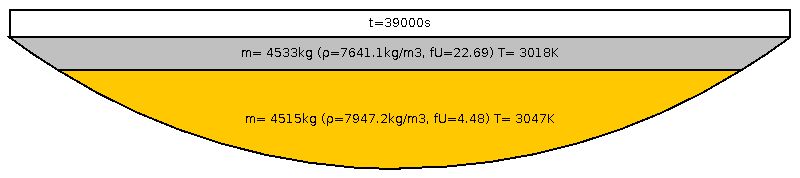
\includegraphics[width=0.85\textwidth, keepaspectratio=true]{Figures/coriumPool_t=39000.png}
\caption{Les différentes stratifications quasi-stationnaires du bain de corium en fond de cuve atteintes lors du test : \textcolor{yellow!75!black}{\textbf{OX.}} à t=0 s puis \textbf{HM.}/\textcolor{yellow!75!black}{\textbf{OX.}} à t=16000 s puis \textcolor{yellow!75!black}{\textbf{OX.}}/\textcolor{gray}{\textbf{LM.}} à t=39000 s.}
\label{fig:stratifications_bains}
\end{figure}

Enfin, la croûte est divisée, tout au long du calcul, en 50 mailles. Le résidu d'apparition de la croûte est de 5 mm. Une température constante et uniforme de 1800 K est imposée sur les parois exterieures de la croûte (seul le couplage entre le modèle de bain de corium et le modèle de croûte sont testés ici).

\subsection{Résultats numériques}


